% 한림대 대학원 학위논문 Latex 양식. made by Jiyong Han, 2021

\documentclass[11pt]{oblivoir}

\hypersetup{hidelinks} % 목차에 빨간 박스 제거

\usepackage{hallym}

\usepackage[a4paper,left=30mm,right=30mm,top=38mm,bottom=50mm]{geometry}

\usepackage{setspace} % 줄간격 변경
\setstretch{1.6} %1.3 :1.5 % 1.6: 2.0%

\usepackage{graphicx}
% Encoder, decoder 그림
\usepackage{tikz,pgfplots}
\usetikzlibrary{graphs,matrix,positioning,calc,fit,backgrounds,chains}
\usepackage{amsmath}
\usepackage{mathrsfs}
\usepackage{mathtools}
\usepackage{indentfirst}% 첫 문단 들여쓰기

\renewcommand{\contentsname}{목차}
\renewcommand{\listtablename}{표 목차}
\renewcommand{\listfigurename}{그림 목차}

\begin{document}
% 제목 기입
 \KoreanTitle{딥러닝 기반 신호 변조 시스템: 설계와 학습}
 \EnglishTitle{Hybrid Neural Coded Modulation: Design and Training Methods}
%  심사위원 기입
\RefereeChief{고 영 웅}
\RefereeSecond{임 성 훈}
\RefereeThird{노 원 종}
\RefereeFourth{김 태 운}

% 겉표지
\makefrontcover
% 빈 표지
\myemptypage

% 속표지
\makefrontcover

% 심사판 정지
\makeapproval

% 목차 페이지 생성
\tableofcontents
\listoffigures
\listoftables

\newpage

\section{\centering 서론}

\subsection{연구 배경}

기계학습(Machine Learning)을 활용한 인공지능(Artificial Intelligence)기술은 컴퓨터가 주어진 데이터를 분석해 원하는 형태의 결과를 도출하도록 스스로 학습하는 알고리즘으로 현재 영상처리, 자연어처리, 신호처리 및 여러 분야에 적용되어 기존 알고리즘 성능의 한계를 돌파하며 다양한 성과를 달성하고 있다~\cite{oshea--hoydis2017}. 무선 통신의 채널 코딩~\cite{faruque2016introduction}영역 또한 기계학습 알고리즘을 활용한 연구~\cite{Balevi--Andrews2020}가 활발하게 진행되고 있는 분야로 다양한 문제를 해결하고, 불완전한 오류 정정 알고리즘을 개선하고 있다..........

\subsection{관련연구}

채널 코딩에서 딥러닝 학습을 사용한 여러 연구 사례~\cite{oshea--hoydis2017,jiang--kim--asnani--kannan--oh--viswanath2020,kim2020,Shental2019,Koike-Akino--Wang--Millar--Kojima--Parsons2019}가 존재한다. 본 논문은 전체 채널 코딩 과정에서 선형 코드를 사용한 채널 부호화, 복호화 과정과 신호 변복조를 분리하여 신호 변복조 과정을 딥러닝으로 학습한 신경망으로 대체하는 연구를 수행한다.

~\cite{oshea--hoydis2017}는 심층 신경망을 학습하여 채널 코딩의 전체 과정을 end to end 형태로 대체하려는 시도를 하였으나 전송하는 코드의 길이가 매우 짧은 7,4 Hamming code~\cite{7955265} 에 대해 연구를 수행하였다. 전송하는 코드(codeword)의 길이에 따라 전송 가능한 전체 codeword의  수가 기하급수적으로 증가하기에 실제 환경에서 적용할 수 없지만 채넗 코딩 기술에 딥러닝 학습을 적용하는 개념을 도입하였다.......

\newpage

\section{\centering 기계학습 및 딥러닝}
\subsection{기계학습}

기계학습은 데이터들의 분포를 원하는 문제에 맞춰 특정 분포로 표현할 수 있는 모델(함수)를 찾는 절차로 크게 학습, 검증, 평가 단계로 분리된다. 기계학습은 수집한 데이터들을 기반으로 발생 가능한 모든 경우에 대해 일반화가 잘 된 모델을 찾는 것을 목표로 한다.......

\subsection{심층 신경망 및 활성화 함수}

\begin{figure}[h!]
    \centering
    \DrawDNN
    \caption{심층 신경망; DNN(Deep Neural Network)}
    \label{fig:my_label}
\end{figure}

인공 신경망, ANN(Artificial Neural Network)~\cite{McCulloch1990ALC}은 딥러닝의 기반으로 인간의 신경 세포를 모방한 구조에서 착안되었다.......

\begin{figure}[h!]
\vspace{2em}
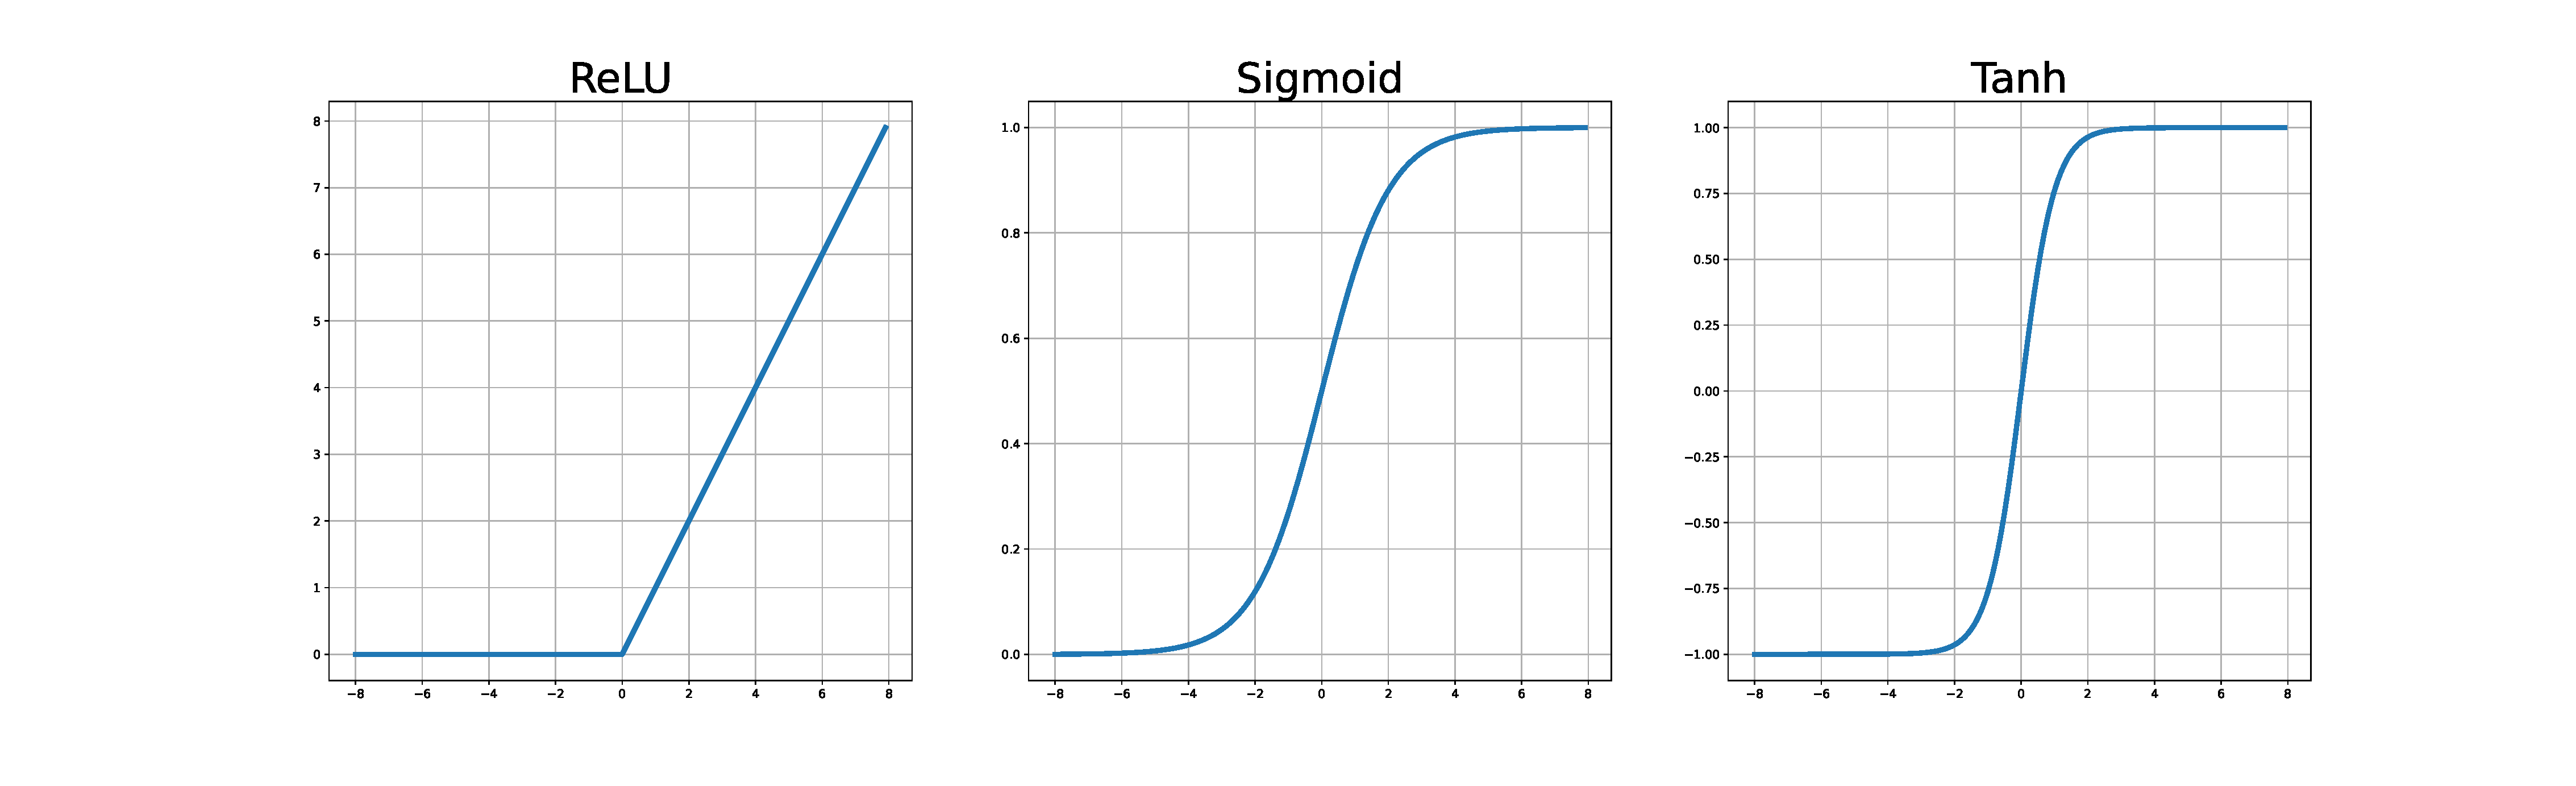
\includegraphics[width=1\columnwidth]{figure/activation.eps}
\vspace{2em}
\caption{활성화 함수 : ReLU, Sigmoid, Tanh}
\label{fig:activation}
\end{figure}

해당 논문에서는 ReLU(rectified linear unit)~\cite{nair2010rectified}, Sigmoid, Hyperbolic Tangent 활성화 함수를 사용하며 그림 2는 각 함수들을 그리고 있다.......

\newpage

\section{\centering 채널 코딩 :Channel Coding}

채널코딩~\cite{faruque2016introduction}은 무선 이동통신 시스템에서 bit 단위의 디지털 신호의 오류를 검출, 정정하는 과정을 의미하며 채널 부호화, 채널 복호화 과정을 합쳐 채널코딩으로 칭한다....

\subsection{반복 코드 :Repetition Code}

반복 전송 코드(Repetition Code)는 오류 정정을 위해 추가 정보를 덧붙여 전송하는 가장 기본적인 방식으로....

\subsection{Hamming 74 Code}

Hamming code~\cite{7955265}는 1950년 미국 Bell 연구소의 Hamming이 고안한 간단한 선형 블록 부호이다.... 

\newpage

\subsection{Interleaving in 5G Code}

\subsubsection{Gray Code}

\begin{table}[h!]
\footnotesize
\centering
\caption{BCD , GCD}
\begin{tabular}{@{}lcc@{}}
\toprule
Decimal& BCD(Binary Coded Decimal) & Gray code\\ \midrule
0 & 0000 & 0000\\
1 & 0001 & 0001\\
2 & 0010 & 0011\\
3 & 0011 & 0010\\
4 & 0100 & 0110\\
5 & 0101 & 0111\\
6 & 0110 & 0101\\
7 & 0111 & 0100\\
8 & 1000 & 1100\\
9 & 1001 & 1101\\
10 & 1010 & 1111\\
11 & 1011 & 1110\\
12 & 1100 & 1010\\
13 & 1101 & 1011\\
14 & 1110 & 1001\\
15 & 1111 & 1111\\
\bottomrule
\end{tabular}
\label{tab:GrayCode}
\end{table}

QAM에서는 그레이 부호(Gray Code)~\cite{doran2007gray}를 사용하여 성운도를 배치한다. 그레이 부호~\cite{doran2007gray}는 순차적으로 증감하는 경우에 전후로 한 bit만 변경하면 되는 특징을 갖고 있다. 이 특징을 사용하여 QAM에서의 성운도는 인접한 bit들이 모두 하나의 bit만 차이나도록 배치되어 있다. 이러한 배치로 채널을 통과하며 잡음이 더해진 신호의 복호력을 강화할 수 있다.

\begin{figure}[h!]
\footnotesize
\centering
\DrawInterleaving
\caption{5G  LDPC code Interleaving}
\label{fig:system}
\end{figure}

5G LDPC 코드에서 사용되는 interleaver~\cite{bae2019overview}는 행과 열을 기준으로 변환된다. 행의 크기는 변조 차수를 기준으로 4,16,64,256 QAM에 의해 결정된다. codeword의 길이가 $E$인 경우, $\log \text{변조 차수}$를 기준으로 $M \times E/M$으로 변환 후 위에서 아래로 codeword를 재배열하는 방식이 사용된다. 이런 방식을 사용하는 이유는 그레이 부호를 사용하여 배치한 QAM의 성운도에 있다. LDPC 인코딩이 적용된 codeword는 메세지 정보를 담는 bits, 오류 정정을 위한 parity check bits 순서로 배치되어 있다. 그림 12의 QAM 성운도를 참고하면 그레이 부호를 사용한 배치의 성운도는 인접한 심볼이 하나의 bit만 차이나며, 중앙을 기준으로 MSB(Most Significant Bit)에 대한 오차 발생률이 $50 \%$가 된다. 즉, 나머지 bit들에 비해 높은 보호력을 갖기 때문에 전송하고자 하는 정보bit를 심볼의 첫 번째 bit에 배치하기 위해 interleaver~\cite{bae2019overview}를 사용한다.

\newpage

\section{\centering 딥러닝 기반 신호 변조}

\subsection{실험 환경}

채널 코딩~\cite{faruque2016introduction}은 선형 부호 코드와 신호 변조의 조합으로 사용되고 있다. 본 실험에서는 QAM 기반 신호 변조 과정을 심층 신경망으로 대체한다.....

\begin{figure}[h!]
\footnotesize
\centering
\DrawCommunicationSystem
\caption{AWGN 채널 모델을 사용하는 통신 시스템}
\label{fig:system}
\end{figure}

\subsection{신경망을 활용한 신호 변복조}

\begin{figure}[h!]
\footnotesize
\centering
\DrawBicmArchitecture
\caption{Bit interleaved coded modulation system architecture.}
\label{fig:system}
\end{figure}

그림 15는 BICM(Bit Interleaved Coded Modulation)~\cite{caire--taricco--biglieri1998, Martinez--Guillen--Caire--Willems2009} 시스템 구조를 기반으로 신경망과 선형 코드의 조합을 나타낸다....

\subsection{GMI를 통한 최적화}

신경망을 학습하기 위한 오차 함수로 GMI~\cite{Merhav1994, Martinez--Guillen--Caire--Willems2009}를 변형하여 사용한다. 

\begin{align}
    I^{gmi}(X;Y) &= E\left[\log\frac{q(X, Y)}{\sum_{x'\in X }P_X(x')q(x', Y)}\right]\\
    \hat{I}^{gmi}(X;Y) &:= E\left[\log\frac{q(X, Y)}{\sum_{x'\in C_{\mu} }P_X(x')P_{Y|X}(Y|x')}\right]\\
    &=M +E\left[\log\frac{q(X, Y)}{\sum_{x'\in C_{\mu} }P_{Y|X}(Y|x')}\right]\\
    &=M+E\left[\log\frac{\prod_{i=1}^m q(C_i, Y)}{\sum_{x'\in C_{\mu} }P_{Y|X}(Y|x')}\right]
\end{align}


\subsection{학습 방법}

본 논문에서는 5G 표준 LDPC 코드에서 첫 번째 Base graph($46 \times 68$), $Z_c$(Expansion Factor) = 24, 코드 전송 비(Code Rate)은 $\frac{1}{2}$인 코드를 사용한다. 위 조건에서 전송하는 정보의 길이는 $528 bits$로 $H$(Parity Check Matrix)로 인코딩 되어 $528\times1104$의 크기로 전송하는 codeword를 puncturing 후 $1104-2*Z_c(2\times 24)= 1056$를 전송한다.
디코딩에서 SPA~\cite{kschischang2001factor}의 최대 반복 수는 50번으로 실험하였다. 심층 신경망의 학습은 실제 성능 평가와 독립적으로 진행되며 변조 차수에 맞춰 학습에 사용되는 symbol은 랜덤하게 생성한다. 성능 평가에서는 LDPC코드로 인코딩 된 codeword를 symbol으로 분리 후 전송하여 신경망을 통과, 다시 합친 후 디코딩하여 오류를 측정한다.

\begin{table}[h!]
\footnotesize
\centering
\caption{DNN training parameters for 1st stage and 2nd stage training.}
\begin{tabular}{@{}lcc@{}}
\toprule
Parameters & $M=16$ & $M=64$ \\ \midrule
Enc. hidden units                 & $[16, 64,  32]$        & $[64, 128, 128, 128]$        \\
1st stage dec. hidden units           & $[128]$      & $[128]$        \\
2nd stage dec. hidden units           & $[128]$         & $[64, 128]$         \\
Training $\SNR$           & $7$ dB      & $11.5$ dB        \\
1st stage batch size           & $M\times 20$      & $M\times 20$        \\
2nd stage batch size           & $M\times 1600$         & $M\times 1600$         \\
Number of samples           & $M\times 4800$      & $M\times 3200$        \\
Learning rate              & $[0.1\sim 0.001]$       & $[0.1\sim 0.001]$        \\
1st stage optimizer              & AdamW (0.01)       & AdamW (0.2)        \\
2nd stage optimizer              & Adam       & Adam        \\
Activation functions  & $\tanh$, ReLU    & $\tanh$, ReLU        \\ 
%Scheduling & cosine annealing & cosine annealing\\
\bottomrule
\end{tabular}
\label{tab:dnn}
\end{table}

최적화를 위해 학습은 사전 단계와 본 학습, 두 단계로 나눠 진행한다. 테이블 1은 각 단계별 학습에서 사용되는 하이퍼 파라미터를 표시한다. 첫 번째 학습에서는 작은 batch 크기와 $L_2$ 규제화를 포함하는 AdamW~\cite{loshchilov--hutter2018} 최적화 함수를 사용하여 인코더가 성운도의 모양을 학습 할 수 있도록 한다. 성운도의 모양이 수렴되면 두번째 학습 단계에 전달한다. 본 학습 단계는 전이학습을 통해 가중치 미세조정(fine-tuning)으로 신경망의 최적화를 수행한다. 첫번째 학습 단계에서의 인코더는 유지하고 디코더는 보다 복잡하게 설계하여 큰 배치의 데이터와 규제화를 사용하지 않는 Adam 최적화 함수를 사용하여 학습한다. 

\subsection{성능 평가}

\begin{figure}[h!]
    \centering
    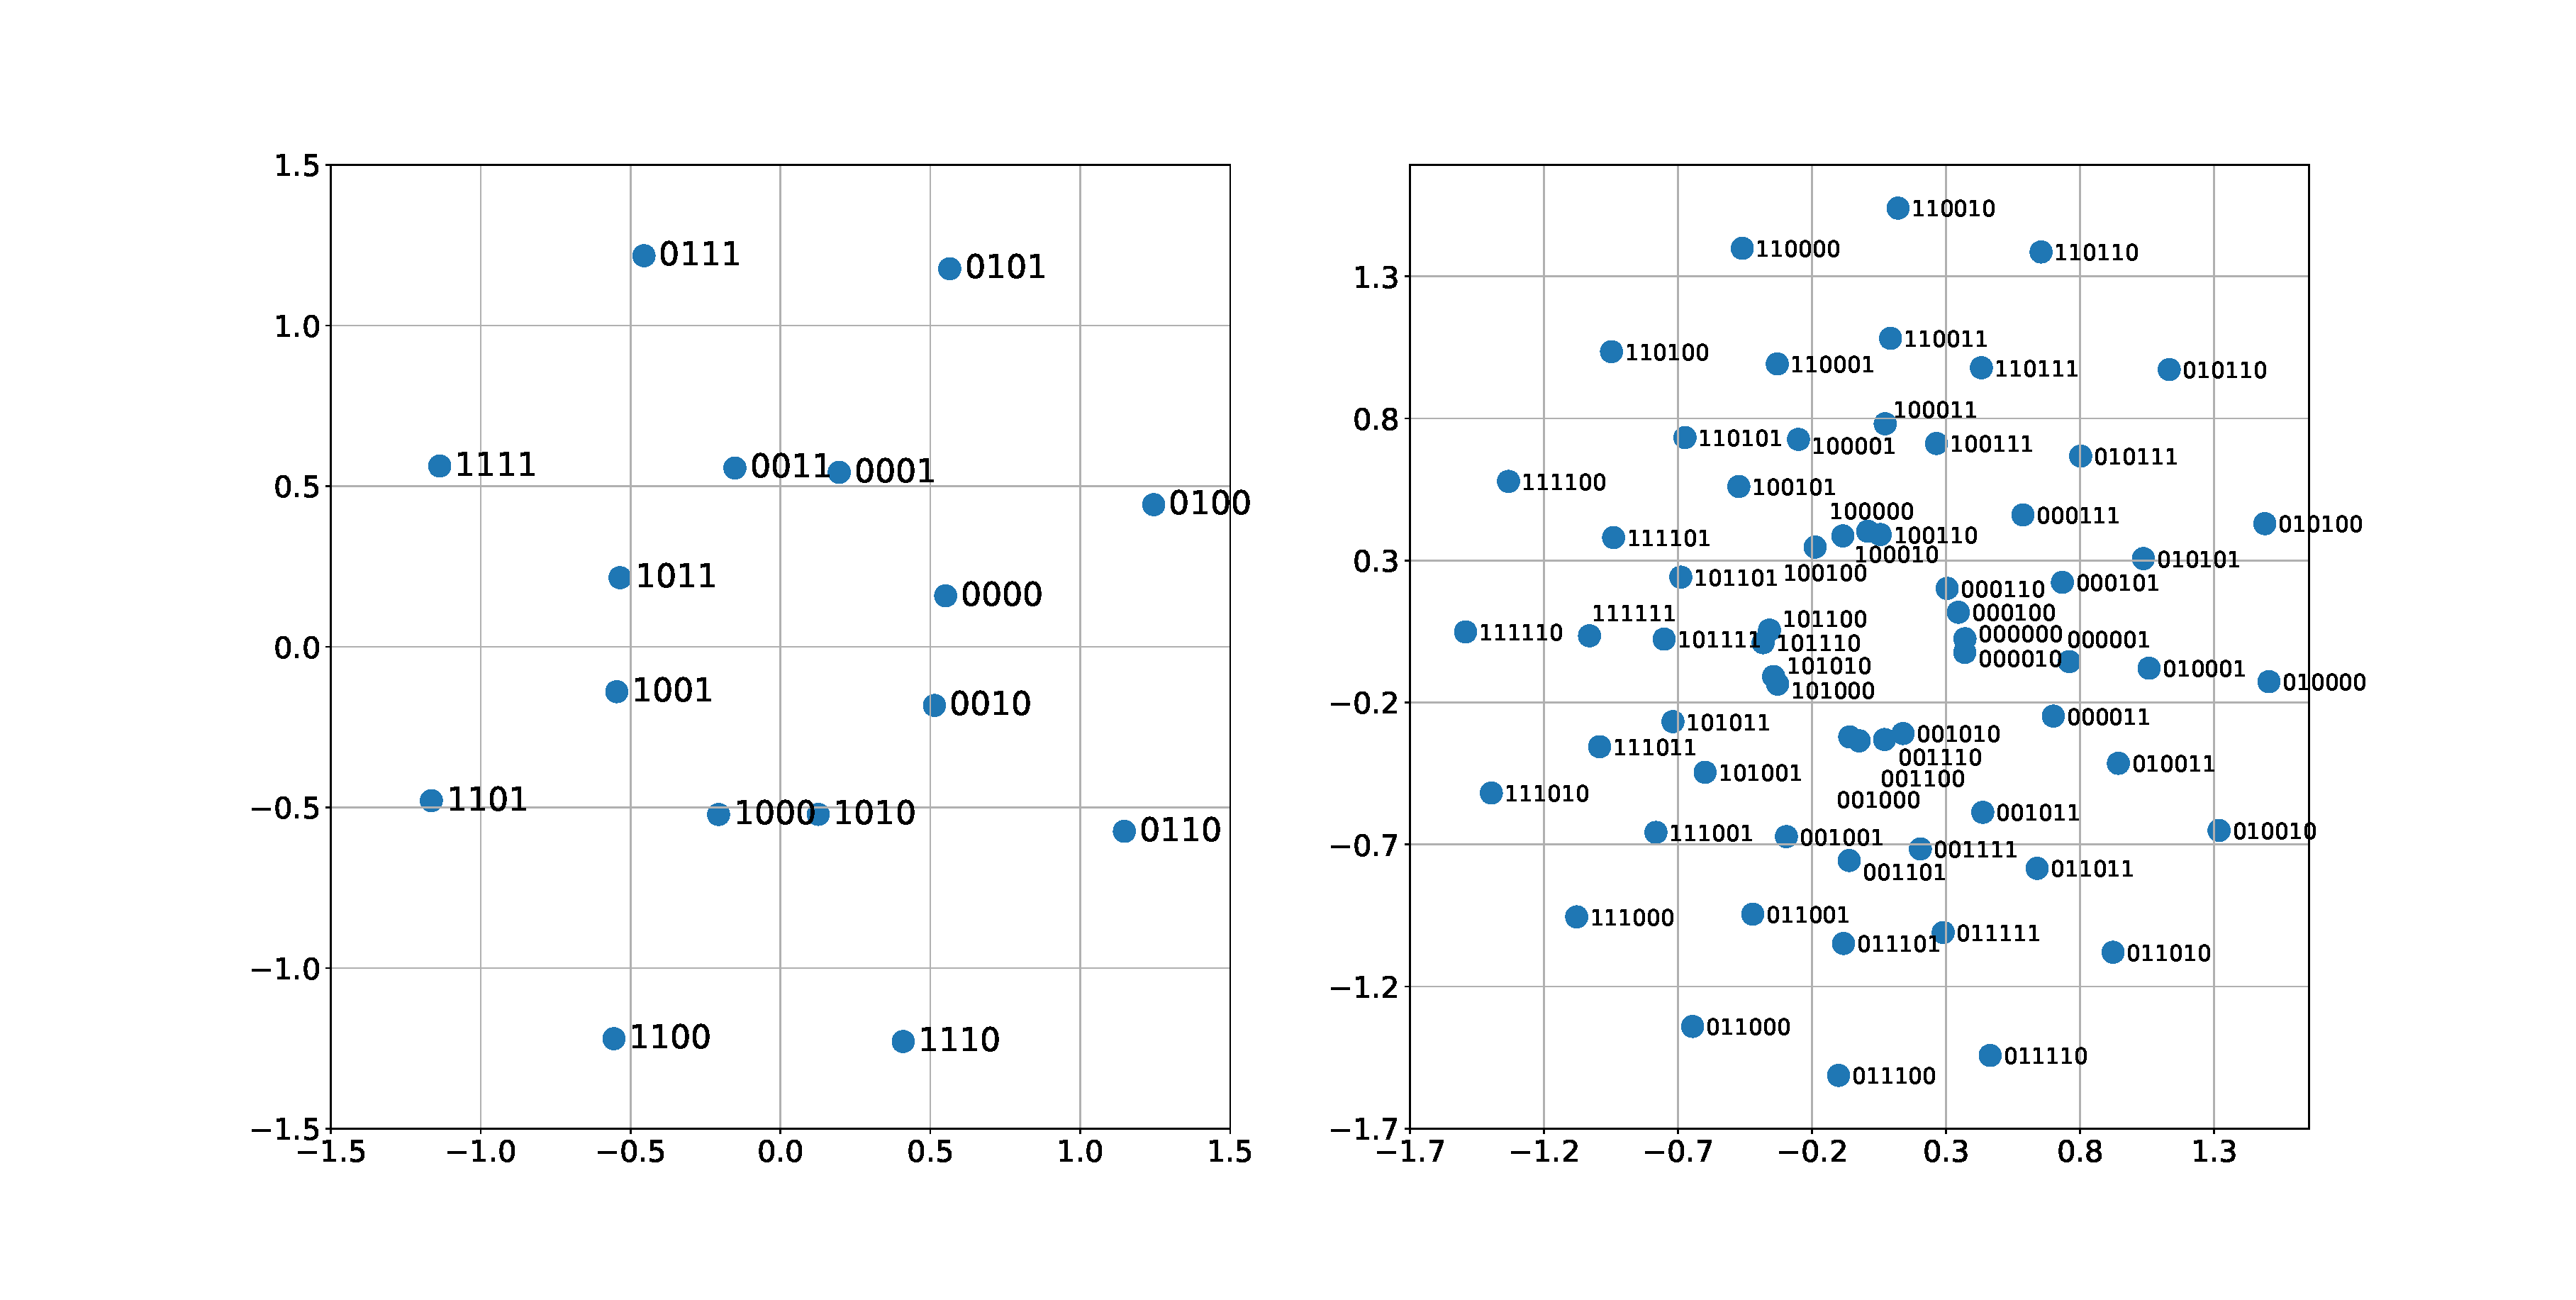
\includegraphics[width=1.\columnwidth]{figure/DNNconstellations.eps}
    \caption{심층 신경망으로 학습한 16,64 성운도}
    \label{fig:my_label}
\end{figure}

그림 16은 변조 차수 $M \in {16,64}$에서 학습한 성운도를 나타낸다. 그림12의 QAM 성운도에 비해 AWGN 채널에 맞는 가우시안 분포의 모양을 띄고 있다. 또한 딥러닝 학습으로 얻은 성운도의 symbol 배치가  최상위비트(MSB; Most significant Bit)가 좌우 대각선을 기준으로 구분되는 gray mapping을 따르고 있다.

\begin{figure}[h!]
    \centering
    \DrawError
    \caption{QAM, DNN 성능 비교}
    \label{fig:my_label}
\end{figure}

그림 17은 QAM과 신경망을 사용하였을때 성능을 비교한다. 그림에서 보여지는.........

\newpage


\section{\centering 결론}

본 논문은 Shannon이 증명한 이론적인 최대 채널 용량을 도달하지 못한 채 사용되고 있는......

%Reference 페이지 생성: ieeetr 옵션: 본문에 등장한 순서대로 
\bibliographystyle{ieeetr} 

\clearpage
\bibliography{reference} % .bib 파일 명을 기입하면 된다. 
\cedp

\newpage

\makeabstractKor % 국문 초록 생성

무선 통신의 물리계층에서 사용되는 채널 코딩은 Shannon이 제안하는 구조를 기반으로 구성되어있다. 그러나 Shannon이 증명한 이론적인 최대 채널 용량을 현실에서 구현하는 것이 불가능하기 때문에, 채널 코딩의 인코딩, 디코딩 영역에 특정 구조를 적용하여, 실제 시스템에 적용 가능하면서도, Shannon의 채널 용량에 최대한 접근하도록 하는 방법을 이용하고 있다.....

\\ \\
\textbf{주제어: 딥러닝, 채널코딩, 신호변조, 오토인코더}


\newpage

\makeabstractEng % 영문 초록 생성

The channel coding used in the physical layer of wireless communication is constructed based on the structure proposed by Shannon. .......

\\ \\
\textbf{Keywords: Deep learning, Channel coding, Modulation, Autoencoder}
\end{document}




